%%%%%%%%%%%%%%%%%%%%%%%%%%%%%%%%%%%%%%%%%%%%%%%%%%%%%%%%%%%%
%% Chapter 2 - Fundamentals and Related Work (12-18 pages)
%% Purpose: provide only the theory and literature needed to
%% understand the research choices, then end with the
%% unresolved gap addressed by the thesis.
%%%%%%%%%%%%%%%%%%%%%%%%%%%%%%%%%%%%%%%%%%%%%%%%%%%%%%%%%%%%
\chapter{Fundamentals and Related Work}
\label{chap:fundamentals}

Chapter~\ref{chap:introduction} argued that precise task-space tracking
with a hydraulic mowing arm is limited less by kinematics than by the
actuator. The path from a valve command to actual cylinder motion is
nonlinear and load dependent, and it differs from one machine, season, or
attachment to the next. This chapter collects the background needed to
judge that argument and to understand the design decisions made later in
the thesis. Section~\ref{sec:fund:actuation} introduces the machine class
and its electro-hydraulic actuation. Section~\ref{sec:fund:kinematics}
recalls the kinematic tools behind the classical controller, and
Section~\ref{sec:fund:conventional-control} reviews how conventional
model-based control deals with hydraulic uncertainty. The remaining sections cover the learning methods this work builds on.
Section~\ref{sec:fund:learned-dynamics} treats data-driven dynamics models and
the pitfalls of identifying them from closed-loop data.
Section~\ref{sec:fund:rom} covers reduced-order and grey-box modelling,
Section~\ref{sec:fund:domain-randomization} domain randomisation and latent
adaptation, and Section~\ref{sec:fund:rl-residual} policy optimisation with
structured priors.
Section~\ref{sec:fund:gap} then states the gap that remains and how the
three control stacks of this thesis (\ppoROM, \ppoIDFD, and
\ppoAAMFD) address it. As defined in Chapter~\ref{chap:introduction},
the first two abbreviate PPO--ROM and PPO--ID--FD; AF denotes the deployed
Adaptive Forward stack rather than the offline AAM. Only material that is
needed for the later chapters is included. Background and results are kept
apart: where a later measurement is the reason a line of work was left behind,
it is quoted forward and marked as such, and no argument in this chapter rests
on it. The concrete system definition and problem formulation follow in
Chapter~\ref{chap:system}.

\section{Manipulator Actuation and Control Fundamentals}
\label{sec:fund:actuation}

\subsection{Application Context and Implement Carriers}

The MULAG FME~500 mounts a multi-link hydraulic boom and a
$\unit[1.2]{m}$ flail head on a Unimog carrier~\cite{mulag2026fme500}.
It reaches about $\unit[6.5]{m}$ laterally, below road level and over
obstacles, while an operator adjusts cutter height, tilt and lateral position
as the vehicle moves. Automating this continuous tracking task is the practical
motivation of the thesis.

Hydraulic cylinders suit the required force, shock tolerance and existing
vehicle power supply, but their command gain changes strongly with load and
configuration. This trade-off between force density and precision is central
to hydraulic manipulator control~\cite{mattila2017survey}.

\subsection{The Electro-Hydraulic Actuation Chain}
\label{sec:fund:actuation-chain}

\begin{figure}[H]
  \centering
  \begin{tikzpicture}[x=1cm,y=1cm,>=Latex,font=\small]
  % Match Figure 2.4: one pale framed panel, compact filled blocks and
  % unobstructed semantic-colour arrows.
  \node[draw=cbblue!90!black,line width=.8pt,rounded corners=3pt,
    fill=cbblue!6,minimum width=13.65cm,minimum height=10.55cm]
    (chainpanel) at (0,-4.55) {};
  \node[font=\normalsize\bfseries,text=cbblue!85!black] at (0,.10)
    {Electro-hydraulic actuation chain};

  \tikzset{
    chainblock/.style={draw=black!55,line width=.8pt,rounded corners=2pt,
      minimum width=6.65cm,minimum height=1.08cm,text width=6.15cm,
      align=center,font=\small\bfseries},
    groupname/.style={font=\scriptsize\bfseries,align=center}
  }

  \node[chainblock,draw=cbblue!90!black,fill=cbblue!42]
    (command) at (0,-1.00)
    {valve command $u$\\[-1pt]\footnotesize normalized electrical input};

  \node[chainblock,draw=cborange!90!black,fill=cborange!86]
    (valve) at (0,-2.55)
    {proportional 4/3 valve\\[-1pt]\footnotesize spool $x_v$; flows $Q_A,Q_B$};
  \node[chainblock,draw=cborange!90!black,fill=cborange!72]
    (chambers) at (0,-4.10)
    {cylinder chambers\\[-1pt]\footnotesize pressures $p_A,p_B$; fluid compliance};
  \node[chainblock,draw=cborange!95!black,fill=cborange!90]
    (cylinder) at (0,-5.65)
    {hydraulic cylinder\\[-1pt]\footnotesize stroke $x$; force $F_h$};

  \node[chainblock,draw=cbgreen!90!black,fill=cbgreen!78,text=white]
    (linkage) at (0,-7.20)
    {boom linkage\\[-1pt]\footnotesize configuration-dependent transmission};
  \node[chainblock,draw=cbgreen!90!black,fill=cbgreen!68,text=white]
    (head) at (0,-8.75)
    {mowing head\\[-1pt]\footnotesize task-space pose $\bm{p}_c$};

  \draw[sigarrow,cbblue!90!black] (command) -- (valve);
  \draw[sigarrow,cborange!90!black] (valve) -- (chambers);
  \draw[sigarrow,cborange!90!black] (chambers) -- (cylinder);
  \draw[sigarrow,cbgreen!80!black] (cylinder) -- (linkage);
  \draw[sigarrow,cbgreen!80!black] (linkage) -- (head);

  \node[groupname,text=cbblue!85!black] at (-5.08,-1.00) {ELECTRICAL};
  \node[groupname,text=cborange!85!black] at (-5.08,-4.10) {HYDRAULIC};
  \node[groupname,text=cbgreen!72!black] at (-5.08,-7.98) {MECHANICAL};
\end{tikzpicture}

  \caption{The electro-hydraulic actuation chain from valve command to
  mowing-head motion. The block colors distinguish the electrical, hydraulic
  and mechanical stages; each subtitle identifies the principal quantity
  passed to the next stage.}
  \label{fig:fund:chain}
\end{figure}

In Figure~\ref{fig:fund:chain}, an electrical command moves a proportional
valve spool and meters flow to the cylinder chambers. The orifice
law~\cite{merritt1967hydraulic} makes flow depend on spool position and the
square root of the pressure margin. Valve authority is therefore
load-dependent and directional; overlap creates a dead zone near null and the
spool saturates at large commands~\cite{jelali2003hydraulic}.

Compressibility, changing chamber volume, relief limits, leakage and seal
friction further separate flow from motion. Several of these effects are
non-smooth, while bulk modulus, leakage and friction drift with temperature and
wear. The mechanical linkage then converts cylinder translation through
configuration-dependent lever arms. Chapter~\ref{chap:models} consequently
models the hydraulic realisation in cylinder space, before kinematic effects
are mixed into cutter error.

\subsection{High-Fidelity Simulation as a Data Source}
\label{sec:fund:sim-data-source}

The component-level Simscape plant~\cite{mathworks2024simscape} resolves the
stiff hydraulic dynamics but runs one machine at small integration steps.
Policy optimisation instead benefits from thousands of GPU-parallel
plants~\cite{makoviychuk2021isaac}. The detailed model is therefore used
offline to generate identification data; compact actuator models carry its
behaviour into parallel training, as summarised in
Figure~\ref{fig:fund:simtosim}.

\begin{figure}[H]
  \centering
  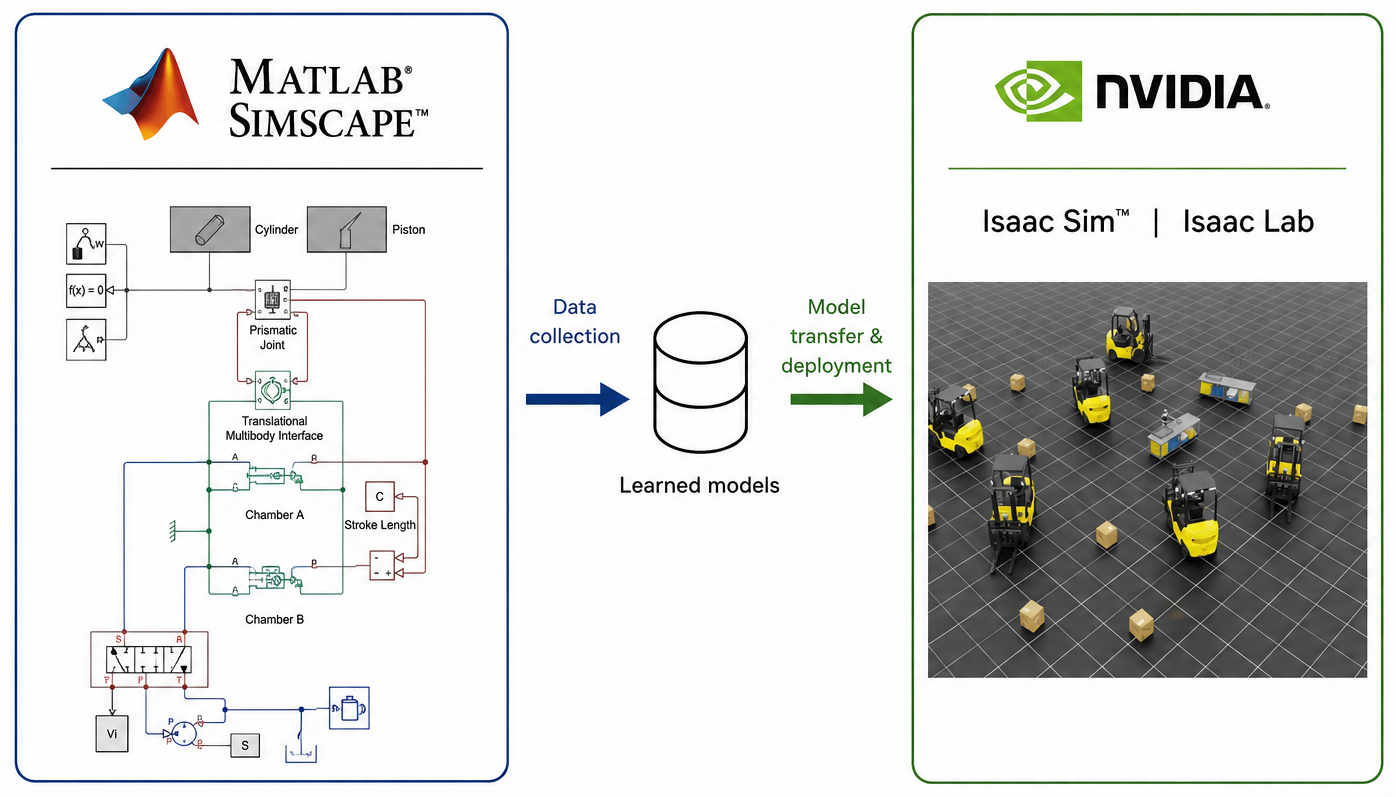
\includegraphics[width=\textwidth]{images/ch2/fund_sim_to_sim}
  \caption{Simscape supplies high-fidelity hydraulic data; compact actuator
  models transfer that behaviour to GPU-parallel training in IsaacLab. Product
  images: MathWorks and NVIDIA.}
  \label{fig:fund:simtosim}
\end{figure}

\section{Kinematics and Task-Space Tracking}
\label{sec:fund:kinematics}

\subsection{Differential Kinematics}

The cutter path is specified in vehicle coordinates, so the manipulator
Jacobian maps joint rates to the required tool velocity
~\cite{siciliano2009robotics}. Near singular configurations the ordinary
pseudo-inverse produces excessive commands. The damped least-squares inverse
of Wampler~\cite{wampler1986manipulator} and Nakamura and
Hanafusa~\cite{nakamura1986inverse} trades some local accuracy for bounded
commands and is retained as the classical controller.

\subsection{From Joint Space to Cylinder Space}

The actuated coordinates are cylinder lengths, and their nonlinear
cylinder-to-joint map has a configuration-dependent lever arm. A passive head
joint further limits independently controllable directions. The calibrated
cutter Jacobian in Chapter~\ref{chap:system} composes these mappings. It still
assumes that commanded cylinder motion is realised; the learned actuator models
address that remaining gap.

\section[Model-Based and Conventional Control Approaches]
  {Model-Based and Conventional Control\\Approaches}
\label{sec:fund:conventional-control}

Three families of conventional control are relevant here: fixed-gain cascades,
nonlinear cancellation, and online parameter estimation. Each of them works on
hydraulic manipulators. Each also carries a maintenance or excitation cost, and
those costs are the reason this thesis learns the actuator instead.

\subsection{Fixed-Gain Cascades}

Industrial implements commonly map joystick input directly to valve current.
The standard improvement is a cascade in which an outer position loop sets a
velocity or pressure reference and a fast inner loop tracks
it~\cite{jelali2003hydraulic}. The construction is cheap, needs no plant model
beyond a few tuned gains, and is what a commercial machine realistically ships
with.

The cost is that the gains are tuned around one operating point. The orifice
law makes command-to-velocity gain scale with the square root of the pressure
margin, so it changes with load and with direction of travel, and the linkage
lever arm changes with configuration. A gain set tuned at the stiff end of that
range responds weakly at the compliant end; tuned at the compliant end it
oscillates at the stiff end. Scheduling the gains over configuration and load
recovers some of the range, but the schedule is machine and attachment
specific and has to be remeasured whenever either changes.

\subsection{Nonlinear Cancellation}

Nonlinear model-based control removes the dependence on an operating point by
cancelling the known dynamics rather than tuning around
them~\cite{slotine1991applied}. For a hydraulic actuator the cancellation has
to span the orifice nonlinearity, chamber compressibility and the rigid-body
load, which places the valve command several integrations away from the
position error and makes backstepping the usual
construction~\cite{jelali2003hydraulic}. The survey of Mattila et
al.~\cite{mattila2017survey} reports this line, together with virtual
decomposition control, as the state of the art for heavy-duty hydraulic arms,
and it does deliver accurate tracking on instrumented machines.

Cancellation is only as good as the model it inverts, and the terms it depends
on are the terms that drift. Bulk modulus, leakage and seal friction change
with temperature and wear over a working day. Some of the structure is
non-smooth and cannot be cancelled at all: valve overlap produces a dead zone
that has to be inverted explicitly, as Yang et
al.~\cite{yang2026stateconstrained} do alongside state constraints. The learned
actuator models of Chapter~\ref{chap:models} carry an explicit dead-zone term
for the same reason. Maintaining this identification per machine, season and
attachment is what makes the family expensive on a commercial
implement~\cite{mattila2017survey}, not any weakness in the control law.

\subsection{Online Parameter Estimation}

Adaptive control estimates the uncertain parameters during operation instead of
fixing them in advance~\cite{astrom1995adaptive}. Yao's adaptive robust control
(ARC) pairs a projection-bounded parameter estimator with a robust feedback
term, so that a guaranteed transient tracking bound does not wait for the
estimate to converge, and it is the established result for single-rod
hydraulic actuators~\cite{yao2000adaptive}. On the face of it this is the
closest classical answer to the problem of this thesis, because it targets
exactly the drifting parameters just described, and because it is the one
classical family that ships a proof rather than an empirical trend, in direct
contrast to the adaptation studied here (Section~\ref{sec:ctrl:af-claims}). ARC
buys that guarantee by assuming a known parametric structure for the plant: the
orifice, chamber and friction terms must be derived correctly in advance, with
only their coefficients left uncertain. That is exactly the assumption
Chapter~\ref{chap:models} finds hard to hold on this machine, where the
reduced-order model's own orifice and friction parameters settle at their
optimisation clamps rather than at physically plausible values
(Section~\ref{sec:models:rom}).

Two properties of the task limit it. Parameter convergence requires persistent
excitation, and mowing supplies smooth, low-bandwidth commands that do not
provide it; the redundancy between command and state that
Section~\ref{sec:fund:identifiability} describes for learned models constrains
a recursive estimator in the same way. The valve also saturates for much of the
scored window on this machine (Section~\ref{sec:models:adapter}), where the
regressor stops reflecting the applied input and adaptation has to be suspended
or explicitly compensated~\cite{sofrony2024antiwindup}. Both limits belong to
the task rather than to the estimator, so they bear on any correction applied to
the command on this machine. They are measured
(Section~\ref{sec:models:adapter-null}) rather than assumed away, and they are
part of why the deployed mechanism conditions the policy instead of correcting
its command.

The scope of that argument should be stated plainly. No classical adaptive
baseline is run in this thesis. The experiments of
Chapter~\ref{chap:evaluation} compare actuator representations inside one
reinforcement-learning stack, so nothing here shows that adaptive robust
control tracks worse than the learned route on this machine. What is claimed is
narrower: the two conditions the classical estimator needs, informative
excitation and an unsaturated regressor, are not supplied by the mowing task,
and the maintenance burden the family carries per machine, season and
attachment is the burden the thesis is trying to remove.

The experiment that would settle the comparison is concrete rather than
hypothetical. It needs four things. The first is a per-cylinder
differential-pressure loop, because ARC's estimator is driven by the same
pressure signal this simulation only produces as an uncalibrated model state
(Appendix~\ref{app:pressure-signals}). The second is an open-loop
identification campaign on the physical implement, to fit the orifice and
friction structure ARC assumes rather than the clamped values the reduced-order
model settles on (Section~\ref{sec:models:rom}). The third is a projection bound
and adaptation gain tuned against that identified structure. The fourth is a
second control implementation, run on the same excitation schedule and
evaluation gates as Chapter~\ref{chap:evaluation}, so that the two families are
compared under one protocol rather than one against the literature's reported
numbers for the other. None of that instrumentation exists on the target machine
yet (Chapter~\ref{chap:conclusion}), which is why the comparison is left open
rather than run.

\subsection{What Is Retained}

The classical methods are not replaced wholesale. Kinematics is reliable and is
kept: the DLS controller of Section~\ref{sec:fund:kinematics} acts as teacher
and as the data-collection controller. What is learned is the part the
model-based families struggle to maintain: the mapping from cylinder command to
realised motion, and the policy that issues that command
(Section~\ref{sec:fund:rl-residual}).

\section{Data-Driven System Identification and Learned Dynamics}
\label{sec:fund:learned-dynamics}

\subsection{Learned Forward and Inverse Dynamics}

Robot model learning distinguishes forward models, which predict the next
state from state and command, from inverse models, which predict the command
for a desired transition~\cite{nguyentuong2011model}. Section
~\ref{sec:models:overview} fixes both interfaces. One-step fit is insufficient
when a forward model is recursively rolled out, because small errors compound
~\cite{nagabandi2018neural}. The models here are therefore trained with
multi-step objectives. Probabilistic ensembles represent growing rollout
uncertainty~\cite{chua2018deep}; recurrent architectures instead retain
unobserved pressure and valve history~\cite{hochreiter1997long,cho2014learning},
as used by the reduced-order model.

\subsection{Closed-Loop Identifiability}
\label{sec:fund:identifiability}

Informative identification requires inputs that excite the plant independently
of feedback~\cite{ljung1999system,isermann2011identification}. In closed-loop
data, command and state history are correlated; a flexible predictor can score
well by ignoring the command, and validation from the same distribution will
not reveal the shortcut~\cite{schoukens2019nonlinear}.

That failure occurred here: a closed-loop forward model reached one-step
$R^2\approx0.999$ yet showed almost no command dependence under ablation.
Chapter~\ref{chap:data} therefore uses open-loop valve excitation, and every
learned model is checked with zeroed and shuffled commands. Prediction score
alone is not treated as evidence of control authority.

\section{Reduced-Order Modelling}
\label{sec:fund:rom}

Reduced-order models retain dominant behaviour at lower cost
\cite{benner2015survey}. Here the full Simscape plant is reduced to
per-cylinder extension, velocity and pressure difference. The construction is
grey-box: known structure is embedded so that data fits what remains unknown
\cite{karniadakis2021physics}. As in the structured dynamics network of
Lutter et al. \cite{lutter2019deep}, explicit physical layers improve
interpretability. The hydraulic ROM retains the orifice, pressure and
integration structure; learned terms represent valve realisation,
configuration-dependent load and bounded residuals.

Hwangbo et al.~\cite{hwangbo2019learning} combined analytic rigid-body
mechanics with a learned actuator response, a pattern later scaled in
GPU-parallel simulation~\cite{rudin2022learning}. Yamamori et
al.~\cite{yamamori2026actuator} instead shaped the physical actuator to match
the simulation. A commercial valve and pump cannot be redesigned in that way,
so this thesis learns the hydraulic realisation while PhysX retains the
rigid-body mechanics (Figure~\ref{fig:fund:workflow}).

\begin{figure}[H]
  \centering
  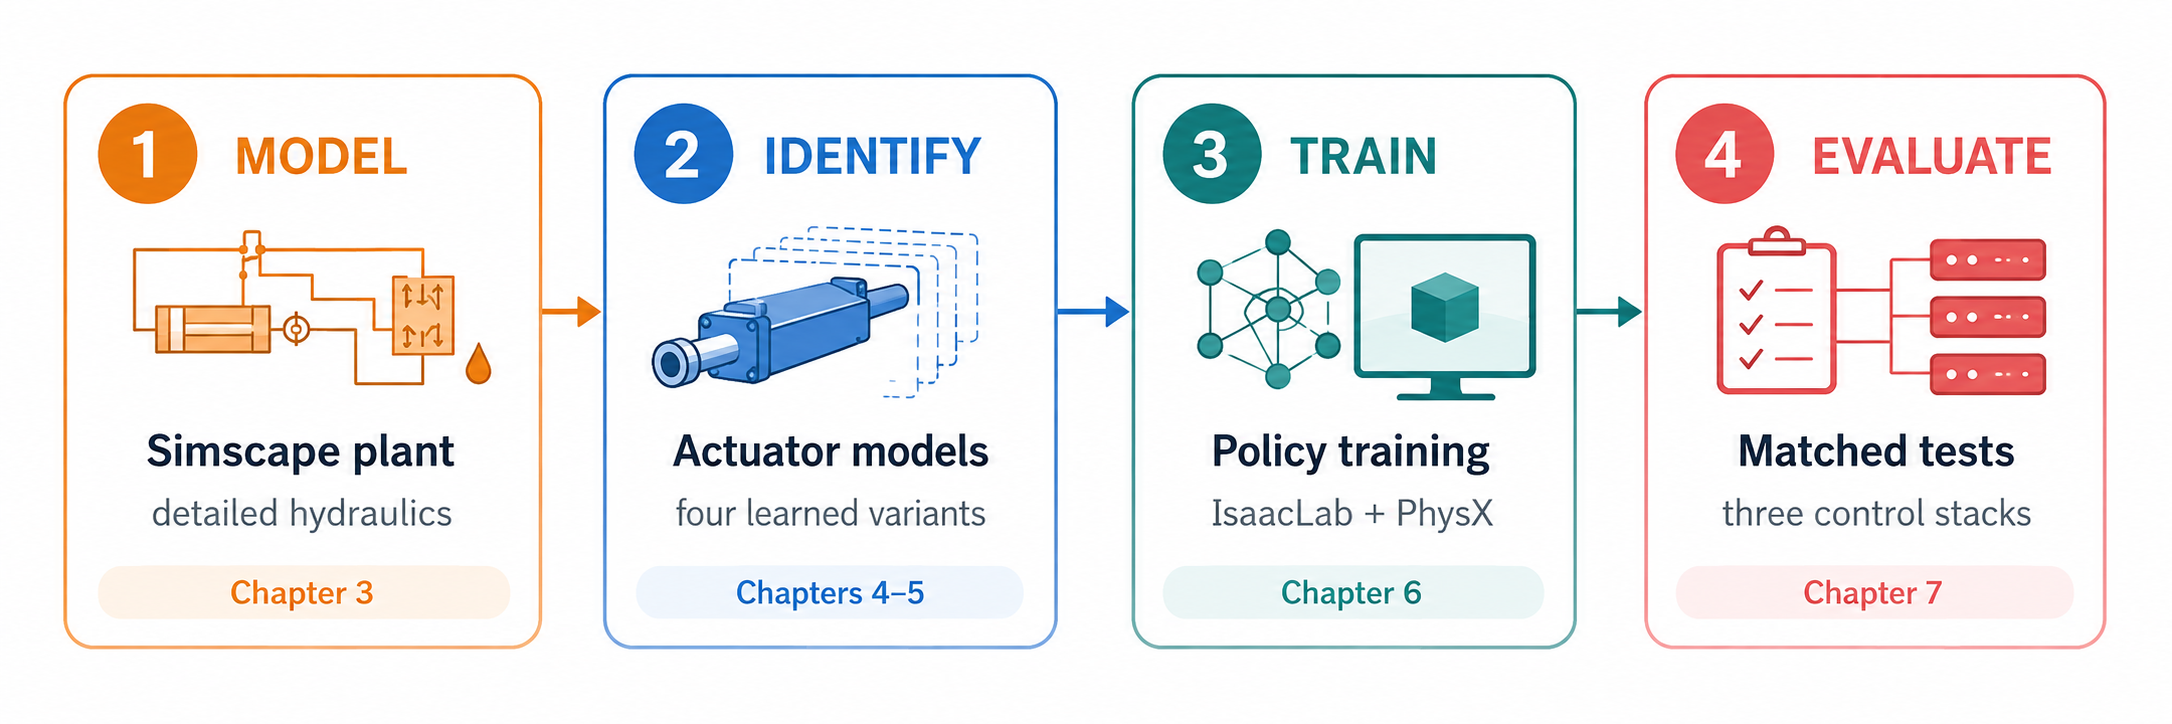
\includegraphics[width=\textwidth]{images/ch2/fund_workflow.png}
  \caption{Workflow from the hydraulic plant model to matched evaluation. The
  separation between rigid-body physics and learned actuation follows the
  actuator-network approach in~\cite{hwangbo2019learning}. This figure was
  generated using AI.}
  \label{fig:fund:workflow}
\end{figure}

\section{Domain Randomisation and Latent Adaptation}
\label{sec:fund:domain-randomization}

\subsection{Robustness Through Randomised Training}

A model trained on one simulated plant inherits its parameters as assumptions.
Domain randomisation instead trains across a family, first for visual
appearance~\cite{tobin2017domain} and then for dynamics such as mass,
friction, gain and latency~\cite{peng2018sim}. The hydraulic family in
Chapter~\ref{chap:data} varies bulk modulus, valve gain, leakage, friction and
payload, producing robustness to physically plausible plant variation.

\newpage
\subsection{From Robustness to Adaptation}
\label{sec:fund:adaptation}

Figure~\ref{fig:fund:robust-adaptive} contrasts a policy trained for one robust
response across the plant family with an adaptive stack that conditions its
response on the current plant.

\begin{figure}[H]
  \centering
  \begin{tikzpicture}[x=1cm,y=1cm,>=Latex,font=\small]
  % Reuse the node colors, line weights and rounded geometry of Figure 3.7.
  \node[draw=cbblue!90!black,line width=.8pt,rounded corners=3pt,
    fill=cbblue!6,minimum width=6.60cm,minimum height=8.55cm] (robustpanel) at (-3.62,-4.05) {};
  \node[font=\normalsize\bfseries,text=cbblue!85!black] at (-3.62,-.25)
    {(a) Robust training};

  \node[draw=cborange!90!black,line width=.8pt,rounded corners=2pt,
    fill=cborange!78,minimum width=5.55cm,minimum height=1.28cm,
    align=center,font=\small\bfseries] (familyR) at (-3.62,-1.45)
    {randomized plant family\\[-1pt]\footnotesize nominal, leakage, stiffness, load};
  \node[draw=cbblue!95!black,line width=.8pt,rounded corners=2pt,
    fill=cbblue!82,text=white,minimum width=5.55cm,minimum height=1.28cm,
    align=center,font=\small\bfseries] (fixed) at (-3.62,-3.75)
    {one fixed policy/model};
  \node[draw=cbgreen!90!black,line width=.8pt,rounded corners=2pt,
    fill=cbgreen!68,text=white,minimum width=5.55cm,minimum height=1.38cm,
    align=center,font=\small\bfseries] (shared) at (-3.62,-6.18)
    {one shared response\\[-1pt]\footnotesize robust across the family};
  \draw[sigarrow,cborange!90!black] (familyR) -- (fixed);
  \draw[sigarrow,cbgreen!80!black] (fixed) -- (shared);
  \node[font=\footnotesize,text=black!62,align=center] at (-3.62,-7.45)
    {same deployed mapping\\for every plant};

  \node[draw=cbblue!90!black,line width=.8pt,rounded corners=3pt,
    fill=cbblue!6,minimum width=6.60cm,minimum height=8.55cm] (adaptpanel) at (3.62,-4.05) {};
  \node[font=\normalsize\bfseries,text=cbblue!85!black] at (3.62,-.25)
    {(b) Latent adaptation};

  \node[draw=cbblue!90!black,line width=.8pt,rounded corners=2pt,
    fill=cbblue!42,minimum width=3.45cm,minimum height=1.05cm,
    align=center,font=\small] (history) at (2.75,-1.30)
    {observable history\\[-1pt]\footnotesize states and commands};
  \node[draw=cbgreen!90!black,line width=.8pt,rounded corners=2pt,
    fill=cbgreen!78,text=white,minimum width=3.65cm,minimum height=1.05cm,
    align=center,font=\small\bfseries] (aam) at (2.85,-2.88)
    {AAM};
  \node[draw=cborange!95!black,line width=.8pt,rounded corners=2pt,
    fill=cborange!86,minimum width=3.65cm,minimum height=1.05cm,
    align=center,font=\small\bfseries] (latent) at (2.85,-4.46)
    {inferred context $\widehat{\bm{z}}$};
  \node[draw=cbblue!95!black,line width=.8pt,rounded corners=2pt,
    fill=cbblue!82,text=white,minimum width=3.65cm,minimum height=1.12cm,
    align=center,font=\small\bfseries] (mapping) at (2.85,-6.10)
    {policy + bounded\\adapter};
  \node[draw=cbgreen!90!black,line width=.8pt,rounded corners=2pt,
    fill=cbgreen!68,text=white,minimum width=3.65cm,minimum height=1.12cm,
    align=center,font=\small\bfseries] (response) at (2.85,-7.72)
    {conditioned response};

  \draw[sigarrow,cbblue!90!black] (history) -- (aam);
  \draw[sigarrow,cborange!90!black] (aam) -- (latent);
  \draw[sigarrow,cbblue!90!black] (latent) -- (mapping);
  \draw[sigarrow,cbgreen!80!black] (mapping) -- (response);

  \node[draw=cborange!90!black,line width=.8pt,rounded corners=2pt,
    fill=cborange!22,minimum width=1.45cm,minimum height=.82cm,
    align=center,font=\scriptsize\bfseries,inner sep=2pt] (teacher) at (5.98,-1.30)
    {training only\\factors $\bm{\xi}$};
  \draw[-{Latex[length=2.0mm]},line width=.8pt,dashed,cborange!90!black]
    (teacher.south west) to[out=-115,in=20] (aam.east);
\end{tikzpicture}

  \caption{Canonical latent-adaptation architecture contrasted with robust
  training. The architecture motivates the offline identifiability study; the
  final AF implementation instead learns its context representation end to end
  from the control objective.}
  \label{fig:fund:robust-adaptive}
\end{figure}

Teacher--student methods encode known simulation factors into a privileged
latent and train an estimator to recover it from observable history. The
construction generalises the wider privileged-learning idea, in which a teacher
with access to unavailable state supervises a student restricted to deployable
observations~\cite{chen2019cheating}. Lee et al.~\cite{lee2020learning} used it
for hidden terrain properties; Kumar et al.~\cite{kumar2021rma} developed rapid
motor adaptation; Miki et al.~\cite{miki2022perceptive} extended the same
teacher--student route to fusing proprioception with exteroception under
unreliable perception. Distillation from a privileged teacher is the mechanism
this thesis uses in Chapter~\ref{chap:control}, with a classical controller in
the teacher's place rather than a privileged
policy~\cite{ross2011reduction}. All of them assume that the factor directions
the estimator retains are the directions the controller needs. Liu et al.~\cite{liu2025frma} report the failure when it
does not hold, where a low-dimensional adapter drops factors that act through
separate channels, and add training phases to recover them. Chapter~\ref{chap:models} finds the same
mismatch here in a sharper form, and the finding is quoted forward because it
is why the deployed stack departs from this line: what an unconstrained
estimate carries here is mainly seal condition, which acts through pressure, and
pressure is the one channel the controller does not integrate
(Section~\ref{sec:models:aam-content}). The deployed controller therefore
conditions on a single physical quantity it can act on, the payload, rather than
on a learned code.

Unlike classical online parameter estimation~\cite{astrom1995adaptive}, the
learned latent need not have a direct physical interpretation. It can be given
one. Hu et al.~\cite{hu2026bayesian} estimate named physical quantities on an
excavator arm with Bayesian reinforcement learning, which buys interpretation
at the price of the explicit plant model that
Section~\ref{sec:fund:conventional-control} identified as the maintenance
burden. The latent used here is anonymous and is therefore audited for content
rather than read as parameters. A latent can also condition a dynamics model
instead of a policy, as in the contextual neural ODE of Yu et
al.~\cite{yu2026context}. That is the nearest relative of the route taken here,
with one difference that decides the outcome: in \ppoAAMFD{} the conditioning
enters the command path rather than the predictor, because a better prediction
helps only if something downstream acts on it.

The offline AAM developed in Chapter~\ref{chap:models} tests whether one second
of observable history contains recoverable plant information. It is not the
encoder deployed in AF, which trains its own history encoder end to end with
the residual under the task objective rather than against an offline target
(Section~\ref{sec:ctrl:af-encoder} details the training scheme). The two routes
therefore answer different questions: the former tests identifiability; the
latter tests control-relevant adaptation. The experiments also keep robust
randomised training distinct from both routes.

Randomised training produces a single controller for a family of plants.
Identification of that family is what makes a member-specific correction
possible. In canonical latent adaptation, adaptation is the online use of that
identification: the controller infers which plant is present from observable
history and conditions the command on that estimate. The two responses are
therefore sequential, not alternatives.

\section{Reinforcement Learning and Structured Priors}
\label{sec:fund:rl-residual}

\subsection{Policy Optimisation}

Reinforcement learning optimises a policy from observations to actions for
expected cumulative reward~\cite{sutton2018reinforcement}. This thesis uses
PPO~\cite{schulman2017proximal} with generalised advantage estimation
~\cite{schulman2016gae}; Section~\ref{sec:ctrl:optimization} gives the exact
objective. GPU-parallel simulation supplies the required throughput
~\cite{makoviychuk2021isaac,rudin2022learning}, which is why compact actuator
surrogates replace the full hydraulic plant during training.

\subsection{Structured Priors for Policy Learning}
\label{sec:fund:prior}

Learning from scratch would discard reliable kinematics. Residual RL instead
adds a bounded learned correction to a controller at runtime
~\cite{johannink2019residual,silver2018residual}. Policy distillation moves the
prior to training: a privileged DLS teacher supplies demonstrations, then the
student acts alone~\cite{ross2011reduction}. This thesis takes the second
route. The teacher is distilled and PPO updates are anchored to the frozen
student (Section~\ref{sec:ctrl:anchored}), and the deployed actor remains the
sole controller: no analytic controller runs underneath it at deployment, so
the runtime correction of residual RL is not the construction used here.

One clarification belongs here, because the vocabulary collides. The adaptive
stack of Chapter~\ref{chap:control} does modify its own frozen actor, but not by
adding a residual in the sense of this subsection. There is no classical
controller beneath it to correct, and its purpose is not to supply a prior that
accelerates learning. It is an online adaptation mechanism internal to the
reinforcement-learning policy, whose only function is to carry the dependence on
inferred plant context that a frozen actor cannot express. It therefore belongs
to the adaptation line of
Section~\ref{sec:fund:adaptation} and is compared against that literature, not
against residual policy learning.

The idea parallels real-world fine-tuning that retains a simulation-trained
value function~\cite{yin2025rapidly}, but here the retained object is the
reference policy. Anchoring was introduced because unconstrained PPO improved
reward while degrading the physical tracking criterion
(Section~\ref{sec:ctrl:training}).

\subsection{Reinforcement Learning on Hydraulic Machines}

Deep RL has reached full-size hydraulic machines. What distinguishes those
stacks from the one built here is not scale but the level at which the policy
commands the machine, because that level decides how much of the hydraulic
chain of Section~\ref{sec:fund:actuation-chain} the policy has to represent at
all.

Egli and Hutter~\cite{egli2020towards} trained an excavator-arm policy in
simulation and transferred it to a full-size walking excavator, then generalised
the construction across excavation tasks~\cite{egli2022general}. The policy
acts on joint-level velocity references, and a low-level tracking layer on the
machine converts them into valve currents. Spinelli et
al.~\cite{spinelli2024rl} keep that division on a commercial material handler
and add an underactuated tool, so the policy has to exploit passive tool
dynamics rather than command them, while the actuated joints are still driven
through the same kind of tracking layer. In both cases the orifice
nonlinearity, the dead zone, the directional asymmetry and the load dependence
live below the learned policy, in a layer that was identified and calibrated for
that machine before the policy existed.

That division is sound where the tracking layer already exists. It is not
available here for two reasons. The FME~500 is a series road-maintenance
implement with no calibrated joint-velocity layer to inherit, and building one
is precisely the per-machine identification that
Section~\ref{sec:fund:conventional-control} identified as the maintenance cost
of the model-based families. More importantly, a velocity interface hides the
quantity this thesis sets out to measure. If the layer beneath the policy
already owns the command-to-motion mapping, the question of whether a learned
actuator retains command authority under saturation and dead zone cannot be
posed at all; it has been answered by construction, once, by hand. The stacks
here therefore command the actuator directly, either as a cylinder increment
realised by a learned model or, in \ppoAAMFD, as the valve command itself.

Maitan et al.~\cite{maitan2026contraction} take the opposite position and train
on the physical cylinder, bounding exploration with a contraction-metric
filter. That work does command the actuator at the low level, and training on
hardware removes the transfer question outright. The result is force control on
a single actuator on a test bench, and it does not obviously scale to a
multi-link boom on a moving carrier, where the exploration the policy needs is
the exploration the filter has to prevent.

These studies settle scale and feasibility. In each of them the actuator
representation is a fixed design choice inside the stack rather than a
variable, so none separates the transfer result from the representation that
produced it. That separation is criterion V below.

None of these stacks varies the plant within a deployment. They are trained for
robustness across one machine and its payload or soil conditions, and a plant
that changes during a run is outside the construction. What remains open is the
combination: a randomised plant family, online actuator adaptation, a
privileged kinematic teacher, and a matched comparison of actuator
representations under one protocol.

A policy can also compensate for a poor actuator model. Chapter
~\ref{chap:evaluation} therefore reports rollout error, command magnitude and
smoothness, and cylinder-level residuals alongside task tracking. Equal task
error alone is not evidence of equal model quality.

\section{Research Gap and Thesis Positioning}
\label{sec:fund:gap}

The literature leaves a specific combination unresolved. Hydraulic control
provides structure but requires maintained plant models; learned dynamics
replace derivation with data but depend on identifiable excitation; actuator
surrogates and latent adaptation are established mainly for electric legged
robots; and hydraulic RL studies do not isolate actuator representation under
a matched protocol. Table~\ref{tab:fund:positioning} summarises this position.

The five criteria are: (I) learned hydraulic actuation, (II) data audited for
causal input identifiability, (III) online adaptation to plant variation at
deployment, (IV) a classical-control prior transferred through policy
distillation, and (V) a matched actuator comparison.

What the table does and does not assert is worth fixing before it is read. The
rows are lines of work, not individual papers, and the criteria are the ones
this thesis needs rather than a neutral taxonomy of the field. Every criterion
is individually established somewhere, several of them for decades, and
single works cover more of a row than a coarse mark can show. The latent
adaptation row in particular samples a large and active literature; it is read
here for the assumption those constructions share, that the factor directions
an estimator retains are the directions the controller needs, and not for
coverage. The claim is the combination on one machine under one protocol, and
Column III shows how narrow even that claim becomes once it is measured rather
than designed for.

\begin{table}[H]
  \centering
  \caption{Positioning against the reviewed lines of work. Parenthesized marks
  denote partial or implicit coverage. Column III is parenthesized for this
  thesis because the deployed route conditions on a single estimated physical
  quantity rather than on the learned latent of
  \cite{lee2020learning,kumar2021rma}, and because its benefit is confined to
  the loaded regime (Section~\ref{sec:eval:adaptation}).}
  \label{tab:fund:positioning}
  \small
  \setlength{\tabcolsep}{3pt}
  \begin{tabular}{@{}p{.69\textwidth}ccccc@{}}
    \toprule
    Line of work & I & II & III & IV & V \\
    \midrule
    \raggedright Model-based hydraulic control\\[-1pt]
      {\scriptsize\cite{mattila2017survey,jelali2003hydraulic}}
      & --- & ($\checkmark$) & ($\checkmark$) & $\checkmark$ & --- \\
    \raggedright Actuator networks for legged robots\\[-1pt]
      {\scriptsize\cite{hwangbo2019learning,rudin2022learning,yamamori2026actuator}}
      & --- & $\checkmark$ & --- & --- & --- \\
    \raggedright RL for hydraulic machines\\[-1pt]
      {\scriptsize\cite{egli2020towards,egli2022general,spinelli2024rl,maitan2026contraction}}
      & $\checkmark$ & ($\checkmark$) & --- & --- & --- \\
    \raggedright Latent online adaptation\\[-1pt]
      {\scriptsize\cite{lee2020learning,kumar2021rma,yu2026context,liu2025frma,hu2026bayesian}}
      & --- & --- & $\checkmark$ & --- & --- \\
    \raggedright Residual RL and policy distillation\\[-1pt]
      {\scriptsize\cite{johannink2019residual,silver2018residual,ross2011reduction,yin2025rapidly}}
      & --- & --- & --- & $\checkmark$ & --- \\
    \midrule
    This thesis (\ppoROM{} / \ppoIDFD{} / \ppoAAMFD)
      & $\checkmark$ & $\checkmark$ & ($\checkmark$) & $\checkmark$ & $\checkmark$ \\
    \bottomrule
  \end{tabular}
\end{table}

Column III carries a parenthesis, and the reason is specific. What
\ppoAAMFD{} deploys is a policy conditioned on one estimated physical quantity,
the payload, recovered online from the task observation it already carries,
rather than the anonymous latent of the canonical architecture.
Section~\ref{sec:eval:adaptation} measures what that conditioning recovers, in
which payload regime it helps, and how much of the gain survives when the
payload is permuted across environments.

The contribution remains the complete experimental chain: identifiable cylinder
data, structurally constrained models fast enough for parallel training, online
adaptation and a common evaluation protocol. Adaptation is reported as a
conditional mechanism, with positive and negative training seeds kept in the
same analysis. The three tested stacks are:

\begin{description}
  \item[\ppoROM.] A command-conditioned ROM realises the policy's desired
    cylinder motion. It is the reference and the only actuator calibrated to
    the deployment plant (Section~\ref{sec:ctrl:constraints}).
  \item[\ppoIDFD.] The same policy interface drives the frozen inverse model
    followed by the strict forward model, forming the robust learned
    baseline.
  \item[\ppoAAMFD.] The policy emits the valve command directly and the
    inverse model leaves the path. A causal history encoder conditions a
    bounded residual on that command, which the same forward model realises
    ahead of PhysX.
\end{description}

All stacks share the task, terrain, trajectories, deployment factors and
evaluation gates. \ppoROM{} and \ppoIDFD{} additionally share the action
contract and form the matched pair; \ppoAAMFD{} does not, because its policy
chooses a valve command rather than a cylinder increment, and it is therefore
compared with its own frozen base rather than ranked against the others. The
ROM is calibrated to the deployment plant, so causal architectural claims rely
on the matched pair and on within-stack paired ablations rather than on a
three-way contrast (Section~\ref{sec:ctrl:matching}). Chapter~\ref{chap:system}
now grounds this comparison in the concrete machine.

The remaining gap concerns the interaction between these established
techniques: whether hydraulic actuators identified for control retain command
authority after transfer, and under which plant conditions a
history-conditioned correction on the identified valve path adds value beyond
randomisation and matched residual capacity.
